\section{Theorie}
\label{sec:Theorie}
\subsection{Einleitung}
Im folgenden Experiment soll das Trägheitsmoment dreier unterschiedlicher Körper bestimmt werden.
Zusätzlich wird ein Körper verwendet, welcher seine Geometrie verändern kann, aber seine Masse beibehält,
wodurch geometrische Beziehungen zum Trägheitsmoment untersucht werden können.

\subsection{Trägheitsmoment \footnote{Unter Verwendung der Quellen \cite{taschenbuch}, \cite{Versuchsanleitung}}}
Analog zur Masse in der Translation wird für Rotationsbewegungen das Massenträgheitsmoment $\symup{I}$ verwendet.
Für eine vollständige Beschreibung der Rotationsdynamik werden zusätzlich die Winkelbeschleunigung $\dot{\omega}$
und das Drehmoment $\symup{M}$ benötigt. Letzteres ist das Äquivalent der Kraft $\symup{F}$ in der Translation.
Im Vergleich wird die Beziehung deutlich
\begin{equation}
    F = m a \quad ,\quad I = M\dot{\omega} \:.
\end{equation}
Dabei gilt für das Massenträgheitsmoment
\begin{equation*}
    I = \sum_i \Delta m_i r_i^2
\end{equation*}
für diskrete und
\begin{equation}
    \label{eqn:integralInertia}
    I = \int r^2 dm
\end{equation}
für infinitesimale Massen.

Da sich \eqref{eqn:integralInertia} aus den Massenabständen bezüglich einer Drehachse errechnet,
ist die Bestimmung für einfache Geometrien nicht aufwendig und meist in Formelsammlungen zu finden.
Bei komplexeren Körpern jedoch ist dies nicht mehr der Fall, sodass dieser mit den einfacheren Geometrien
approximiert wird.
Hilfreiche Referenzen sind Zylinder, dünne, lange Stäbe, Kugeln, Quader und Hohlzylinder, wobei Stäbe und Hohlzylinder
Spezialfälle eines Zylinders darstellen.
\begin{figure}
    \centering
    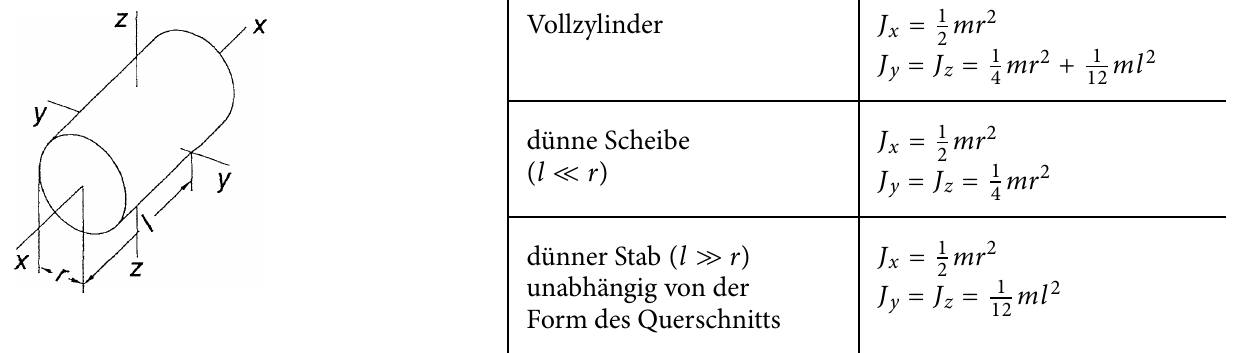
\includegraphics[width=0.9\textwidth]{plots/TrägheitZylinder.png}
    \caption{Das Massenträgheitsmoment eines Zylinders.\cite{taschenbuch}}
    \label{fig:traegZyl}
\end{figure}

\begin{figure}
    \centering
    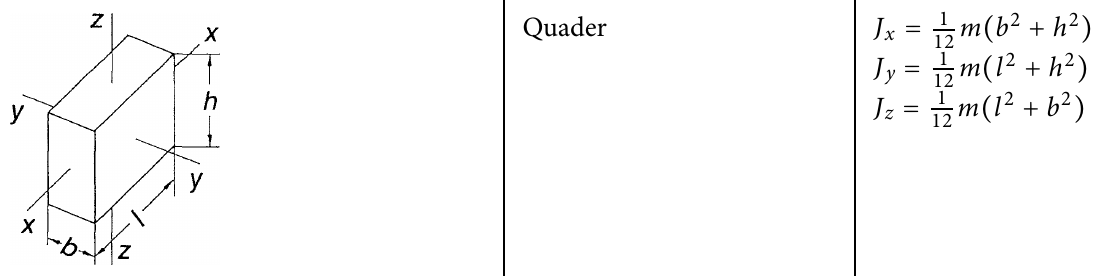
\includegraphics[width=0.9\textwidth]{plots/TrägheitQuader.png}
    \caption{Das Massenträgheitsmoment eines Quaders.\cite{taschenbuch}}
    \label{fig:traegQuader}
\end{figure}

\begin{figure}
    \centering
    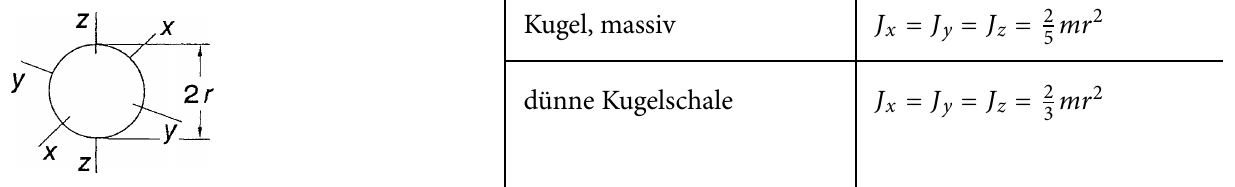
\includegraphics[width=0.9\textwidth]{plots/TrägheitKugel.png}
    \caption{Das Massenträgheitsmoment einer Kugel.\cite{taschenbuch}}
    \label{fig:traegKug}
\end{figure}

In den Abbildungen gilt $J \equiv I$.
Es ist nicht immer der Fall, dass die Rotationsachse auch eine der oben angezeigten Körperachsen entspricht.
Um das Massenträgheitsmoment dennoch ohne aufwendige Integration bestimmen zu können, kann der Steiner'sche
Satz angewendet werden. Wenn $I$ für eine der Trägheitsachsen bekannt ist, kann der gesamte Körper parallel
zu dieser Achse verschoben und mit der Gleichung
\begin{equation}
    I = I_U + ma^2
\end{equation}
berechnet werden. Hier entspricht $I_U$ dem ursprünglichen Massenträgheitsmoment und $a$ dem Abstand zur Achse, um die 
parallel verschoben wird.